\documentclass[../ai_in_finance]{subfiles}
\usepackage[margin=1in]{geometry}
\usepackage{tikz}
\usetikzlibrary{positioning,arrows.meta}
\usepackage{amsmath}
\usepackage{amssymb}
\usepackage{booktabs}
\usepackage{draftwatermark}

\SetWatermarkText{Wulin.Suo@Queensu.ca}
\SetWatermarkScale{1.4}
\SetWatermarkColor{gray!35}
\SetWatermarkAngle{45}

\usepackage{makeidx}
\makeindex

\begin{document}

\chapter{Agent-Based Models in Finance}

\section{Introduction}

Every model in this book so far has taken one of two forms. Chapter 6's machine learning models estimate a function from a fixed dataset, implicitly assuming the data-generating process itself does not change while the model learns from it. Chapter 10's portfolio theory and Chapter 17's reinforcement-learning agents each reason about a single decision-maker, or a small number of them, optimizing against an environment that is either fixed or, at most, adapts slowly. Neither approach is built to answer a question that turns out to matter a great deal in practice: what happens when a large number of participants, each following a simple, individually reasonable rule, interact repeatedly in the same market? Agent-based models\index{Agent-Based Models (ABMs)} (ABMs) answer exactly that question. Rather than solving for an equilibrium in closed form or estimating a statistical relationship from historical data, an ABM specifies a population of heterogeneous agents, each governed by a simple behavioral rule, sets them loose interacting in a simulated market, and treats whatever aggregate pattern emerges, a stable price, a bubble, a crash, a cascade of defaults, as the object of study.

This chapter's central claim is that emergence is the point, not a side effect. Chapter 12's account of the 2010 Flash Crash already described a version of this: no single participant's inventory-management rule was unreasonable in isolation, yet many such rules operating simultaneously produced a collectively destabilizing 
hot-potato effect that no single participant intended or could have predicted from their own rule alone. An ABM makes it possible to reproduce that kind of 
story directly, agent by agent, rather than only describing it after the fact.

Several worked examples run through this chapter, every one of them reproduced in the companion notebook, following the same compute-first 
discipline as every other chapter in this book. A zero-intelligence double-auction example shows that a market mechanism can produce an efficient outcome even when every participant in it behaves close to randomly. A fundamentalist-chartist price-dynamics example shows how the same market can either converge smoothly toward fair value or spiral into a self-reinforcing bubble, depending only on the mix of trading strategies present, with no change to the market mechanism itself, and a 500-period extension of the same model shows fat tails and volatility clustering emerging from nothing more than two simple, fixed behavioral rules switching in and out of dominance. A financial-contagion example, built on the same clearing-vector logic underlying real central-bank stress-testing models, shows a shock to one institution's balance sheet cascading into the default of a second institution that was never directly exposed to the original shock at all, and a second network topology, compared directly against the first under the identical shock, shows that the same total loss can be concentrated into a small number of outright defaults or spread thinly across many surviving-but-weakened institutions, depending only on how the network is shaped. A final pair of examples previews the AI-driven alternative to this chapter's fixed-rule agents, developed in full in Section~\ref{sec:abm-vs-marl}: a seller who learns which of two ask prices is more profitable through repeated trial and error using Chapter 17's own Q-learning machinery, showing the honest limits of trial-and-error learning when an unlucky early experience locks in the wrong lesson, and a fundamentalist-chartist market in which the population mix itself is no longer switched by a threshold the modeler imposes, but by agents comparing each strategy's own recently realized profit through a discrete-choice rule, showing the same bubble-triggering threshold derived earlier in the chapter crossed endogenously rather than by assumption.

It is worth being explicit about where this leaves agent-based models among the three modeling paradigms this book has now covered. Chapter 6's supervised and unsupervised learning models answer the question ``given this data, what function best describes it,'' and are validated by checking predictions against data the model never saw. Chapter 17's reinforcement-learning agents answer ``given this environment, what sequence of actions maximizes reward,'' and are validated by their realized performance, in a backtest or in production. Agent-based models answer a third, different question: ``given these individual rules, what pattern emerges when many such agents interact,'' and, as Section~\ref{sec:abm-calibration} develops at length, are validated far more weakly than either of the other two, by whether a simulated pattern resembles an observed one, not by a held-out prediction or a realized return. None of the three approaches is more fundamentally correct than the others; they answer different questions, and knowing which question a given financial problem actually poses, a prediction problem, a sequential-decision problem, or an emergence problem, is itself one of this book's recurring practical lessons. Table~\ref{tab:abm-paradigms} lays the three side by side.

\begin{table}[htbp]
\centering
\caption{Three modeling paradigms used in this book}
\label{tab:abm-paradigms}
\begin{tabular}{p{2.6cm}p{3.7cm}p{3.7cm}p{3.7cm}}
\toprule
 & Supervised/unsupervised ML (Ch.~6) & Reinforcement learning (Ch.~17) & Agent-based models (this chapter) \\
\midrule
Core question & What function best fits this data? & What action sequence maximizes reward? & What pattern emerges from many interacting rules? \\
Input & A fixed, historical dataset & An environment to interact with & A set of behavioral rules and a market mechanism \\
Validation & Held-out prediction accuracy & Realized backtest or live performance & Resemblance to observed stylized facts (weakest of the three) \\
Typical output & A trained predictive model & A trained policy & A simulated history and its emergent statistics \\
\bottomrule
\end{tabular}
\end{table}

A reader who has followed this book's growing emphasis on machines that learn might reasonably object that every rule described above, zero-intelligence, fundamentalist, chartist, is instead fixed by the modeler in advance, which sits oddly in a chapter that is supposed to belong in a book about AI in finance. That fixed-rule design is a deliberate methodological choice, not a limitation of agent-based modeling as such, and it is one this chapter makes on purpose so that Table~\ref{tab:abm-paradigms}'s third column stays honest: isolating the question of what pattern emerges from a given set of interaction rules from the separate question of how an individual agent's own rule might itself be learned keeps each worked example small enough to hand-check, exactly the same discipline Chapters 1 through 17 already apply everywhere else in this book. That second question, learning the rule itself, is not foreign to this chapter; it is Chapter 17's question, and Section~\ref{sec:abm-vs-marl} connects the two directly. It argues that agent-based models and multi-agent reinforcement learning (MARL) are best read as two different responses to the same limitation Chapter 17 identifies in its own single-agent framing, that training a policy against a fixed historical simulator implicitly assumes every other participant's behavior stays fixed, and it makes the connection concrete through the learning-seller example previewed above, in which one agent in an otherwise fixed-rule market instead learns its own quoting rule through Chapter 17's Q-learning machinery. Every fixed-rule agent elsewhere in this chapter is best read as a transparent, tractable special case of that more general, and considerably harder to train and validate, world in which agents learn rather than follow a rule handed to them, not as a rejection of it.

The chapter's sections follow the same escalating structure in every application: state the mechanism and a small, hand-checkable illustration first, then show what happens when that mechanism is scaled up or repeated many times. Sections~\ref{sec:abm-zi} and~\ref{sec:abm-fundamentalist-chartist} build up market-level price dynamics from individual trading rules, Section~\ref{sec:abm-stylized-facts} scales the latter to hundreds of periods to show real statistical patterns emerging, Sections~\ref{sec:abm-contagion} and~\ref{sec:abm-advanced} apply the identical logic to a network of banks rather than a market of traders, Section~\ref{sec:abm-vs-marl} steps back to compare this chapter's fixed-rule agents directly against Chapter 17's learned alternative, and Section~\ref{sec:abm-workflow} distills the common workflow underlying all of it into an explicit, reusable template before the chapter closes with the practical limitations, summarized in Section~\ref{sec:abm-calibration} and the Challenges section that follows it, that keep agent-based models a specialized complement to this book's other methods rather than a wholesale replacement for them.

\section{Why Agent-Based Models? From Representative Agents to Heterogeneous, Interacting Ones}
\label{sec:abm-why}

Much of classical finance, and much of this book, reasons in terms of a representative agent: Chapter 10's CAPM derives an equilibrium as though a single, rational, mean-variance investor stood in for the whole market; Chapter 7's GARCH models fit a single statistical process to an entire return series without asking which market participants' behavior produced that process. These simplifications are enormously useful, and this book relies on them throughout, but they are also, by construction, unable to answer certain questions. A representative-agent model cannot easily explain why a market that is efficient on an average day can experience a Flash Crash on a particular afternoon, because the average behavior baked into the model has already smoothed away the heterogeneity that made the crash possible in the first place. Agent-based modeling takes the opposite starting point: instead of solving for what a single rational agent would do, it specifies what a whole population of different, typically boundedly rational, agents actually do, and asks what pattern emerges from their interaction.

This bottom-up approach is well suited to exactly the phenomena that are hardest to explain with a representative agent: the fat tails and volatility clustering Chapter 7's GARCH models describe statistically but do not explain mechanistically; asset-price bubbles and crashes that unfold over time rather than instantaneously; and the kind of systemic, contagious risk Chapter 8's stress-testing framework treats largely at the level of a single institution's portfolio rather than as a property of an interconnected system.

Agent-based modeling did not originate in finance. Its most famous early instance is Schelling's\index{Schelling segregation model} (1971) segregation model, built with nothing more sophisticated than a checkerboard and coins of two colors: each agent has a mild preference to have at least some same-type neighbors, far short of wanting to live in a segregated neighborhood, and moves to a nearby empty square only if that mild preference is unmet. Simulating this simple, individually reasonable rule across many agents produces, essentially without exception, a starkly segregated checkerboard, a population-level outcome none of the individual agents' rules asked for or intended. The financial applications in this chapter are the same logic applied to markets rather than neighborhoods: individually reasonable rules, simulated across many interacting agents, producing an aggregate outcome, efficiency, a bubble, a segregated checkerboard, a cascade of defaults, that is a property of the interaction itself rather than of any one agent's intentions.

The idea reached finance specifically through the Santa Fe Institute's Artificial Stock Market\index{Santa Fe Artificial Stock Market}, built in the early 1990s by Arthur, Holland, LeBaron, Palmer, and Tayler, widely regarded as the first serious agent-based model of a financial market. Rather than the two fixed strategy types of Section~\ref{sec:abm-fundamentalist-chartist}'s fundamentalist-chartist model, the Santa Fe market populated its agents with evolving collections of predictive rules, more like a population of simple, competing forecasting models than a fixed behavioral type, and let poorly performing rules die out and successful ones proliferate, an early instance of the same evolutionary, performance-based selection logic Brock and Hommes later formalized more tractably. Its central finding, that this market could switch between a calm, efficient-market-like regime and a volatile, trend-chasing regime depending on how quickly agents adapted their rules, foreshadows exactly the regime-switching mechanism behind Section~\ref{sec:abm-stylized-facts}'s worked example, and the project is generally credited with establishing agent-based computational finance as a distinct research area in its own right, separate from the checkerboard-and-social-science tradition Schelling's model belongs to.

Beyond these historical origins, agent-based models occupy a specific, recurring role in the finance industry today, one this chapter's later sections examine in turn rather than merely assert. Central banks and other macroprudential regulators run network-based ABMs, most prominently the Bank of England's RAMSI discussed in the case vignette below, to stress-test an entire banking system's interconnected exposures rather than one institution's portfolio at a time, now a standard part of the macroprudential toolkit. Exchanges and market-microstructure researchers use zero-intelligence and heterogeneous-agent markets, Sections~\ref{sec:abm-zi} and~\ref{sec:abm-fundamentalist-chartist}'s own subject matter, to understand how much of observed market efficiency, or its breakdown during an event like the Flash Crash, comes from the trading mechanism itself rather than from any participant's sophistication. Quantitative trading desks build synthetic, agent-populated limit-order-book markets to test how a new execution algorithm, of the kind Chapter 11 develops, is likely to move prices and interact with other participants' behavior before ever risking capital on it live, a cheaper and safer proving ground than production trading. And a growing body of academic and industry research combines agent-based markets with the multi-agent reinforcement learning of Section~\ref{sec:abm-vs-marl}, training an execution or market-making policy inside a simulated population of other agents rather than only against static historical data.

Figure~\ref{fig:abm-loop} sketches the basic ABM simulation loop that every example in this chapter follows: a population of agents, each with its own rule, observes the current market state, each agent acts (submits an order, updates a belief, decides whether to pay a debt), those actions are aggregated by a market mechanism into a new market state, and the loop repeats. Nothing here is estimated from historical data the way Chapter 6's models are; everything is specified as a rule and then simulated forward.

\begin{figure}[htbp]
    \centering
    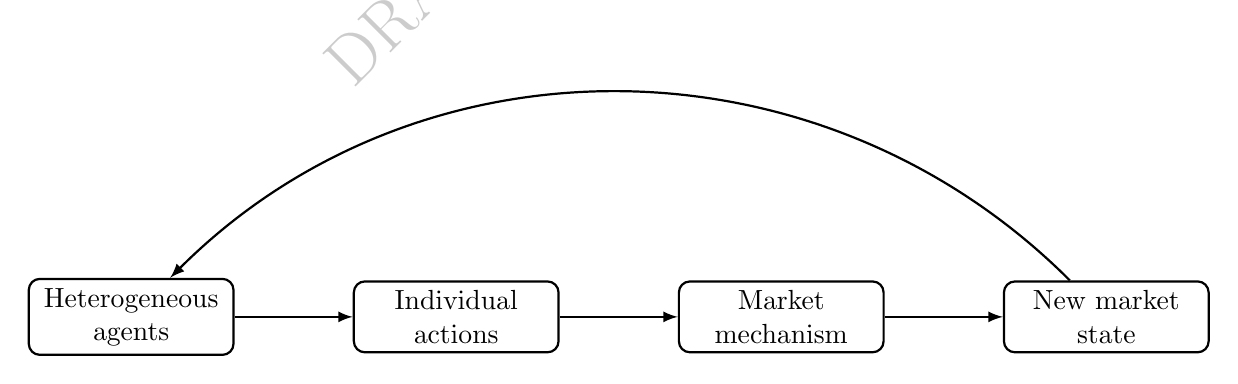
\begin{tikzpicture}[>=latex,thick,node distance=1.5cm]
        \node[draw,rounded corners,minimum width=2.6cm,minimum height=0.9cm,align=center] (agents) {Heterogeneous\\agents};
        \node[draw,rounded corners,minimum width=2.6cm,minimum height=0.9cm,right=of agents,align=center] (actions) {Individual\\actions};
        \node[draw,rounded corners,minimum width=2.6cm,minimum height=0.9cm,right=of actions,align=center] (market) {Market\\mechanism};
        \node[draw,rounded corners,minimum width=2.6cm,minimum height=0.9cm,right=of market,align=center] (state) {New market\\state};
        \draw[->] (agents) -- (actions);
        \draw[->] (actions) -- (market);
        \draw[->] (market) -- (state);
        \draw[->] (state) to[out=135,in=45] (agents);
    \end{tikzpicture}
    \caption{The basic agent-based simulation loop. Each agent observes the current market state and acts according to its own behavioral rule; a market mechanism (a double auction, a price-impact equation, a clearing algorithm) aggregates those individual actions into a new market state, which every agent then observes in the next round. Every example in this chapter is an instance of this loop with a different agent population and market mechanism.}
    \label{fig:abm-loop}
\end{figure}

\section{Zero-Intelligence Traders and the Double Auction}
\label{sec:abm-zi}

The most striking early result in agent-based market modeling, due to Gode and Sunder\index{Gode-Sunder zero-intelligence model} (1993), is that a double auction, the same continuous matching of bids against asks behind the limit order book Chapter 3 introduced, can produce a highly efficient outcome even when every trader in it is, in a precise sense, not intelligent at all: a ``zero-intelligence'' trader submits a bid or ask drawn at random from a budget-feasible range, with no attempt to reason strategically about price or about other traders. Consider two buyers with private valuations $V_{B1}=\$52$ and $V_{B2}=\$48$, and two sellers with private costs $C_{S1}=\$45$ and $C_{S2}=\$50$, for one unit of the same asset each. The efficient allocation, the one a fully rational market would produce, is easy to find directly: buyer 1 and seller 1 should trade, since $V_{B1} > C_{S1}$ generates a surplus of $52-45=\$7$, while buyer 2 and seller 2 should not trade, since $V_{B2} < C_{S2}$ would destroy value. Total efficient surplus is therefore exactly $\$7$.

Now suppose each buyer submits a random bid drawn from $[0, V]$ and each seller a random ask drawn from $[C, 100]$, with no knowledge of anyone else's valuation, and suppose in one simulated round these random draws happen to be $b_1=\$50$ (buyer 1), $b_2=\$30$ (buyer 2), $a_1=\$47$ (seller 1), and $a_2=\$65$ (seller 2). The standard double-auction clearing rule sorts bids from highest to lowest and asks from lowest to highest, then matches and trades every pair for which the bid meets or exceeds the ask:
\begin{align*}
\text{Bids (descending):} &\quad 50, \ 30, \\
\text{Asks (ascending):} &\quad 47, \ 65.
\end{align*}
The top bid, $\$50$, meets the top ask, $\$47$ ($50 \ge 47$), so buyer 1 and seller 1 trade; the second bid, $\$30$, does not meet the second ask, $\$65$ ($30 < 65$), so buyer 2 and seller 2 do not trade. The clearing mechanism has, purely as a byproduct of matching random bids against random asks, selected exactly the efficient pair, buyer 1 with seller 1, and rejected exactly the inefficient one. Whatever transaction price rule is used, for instance the midpoint of the matched bid and ask, $(50+47)/2 = \$48.5$, the realized surplus, computed from the traders' true valuations rather than their randomly drawn bids, is $V_{B1} - C_{S1} = 52 - 45 = \$7$, the full efficient surplus, captured even though neither trader bid or asked anything close to their true valuation. The lesson, confirmed far more systematically in Gode and Sunder's original experiments across many traders and many rounds, is that a market's efficiency can come substantially from the structure of the trading mechanism itself, rather than from the sophistication of the individual traders using it, a genuinely counterintuitive result relative to the fully rational representative agent Chapter 10 builds its equilibrium models around. It is also worth being precise about what this single hand-worked round does and does not establish: it shows the mechanism \emph{can} select the efficient pair from random bids, not that it \emph{always} will, and, as the companion notebook's own supplementary experiments with this same tiny two-buyer, two-seller market confirm, a single random draw from a wide bidding range is in fact a noisy way to reach that outcome; Gode and Sunder's actual, far more robust result relies on many traders and many independent trading opportunities per period, not on any one exchange like the one worked by hand above.

\subsection*{Building a Simple ABM in Python}

Every agent-based model in this chapter reduces to the same two ingredients Chapter 2 already teaches how to code: a data structure representing each agent's state, and a function that updates the market given every agent's action. The zero-intelligence double auction above is only a few lines:
\begin{verbatim}
import random

def zero_intelligence_round(buyers, sellers, seed=None):
    rng = random.Random(seed)
    bids = [(rng.uniform(0, v), v) for v in buyers]      # random bid, true value
    asks = [(rng.uniform(c, 100), c) for c in sellers]    # random ask, true cost
    bids.sort(key=lambda x: -x[0])
    asks.sort(key=lambda x: x[0])
    trades = []
    for (bid, val), (ask, cost) in zip(bids, asks):
        if bid >= ask:
            trades.append({'price': (bid + ask) / 2, 'surplus': val - cost})
    return trades

trades = zero_intelligence_round(buyers=[52.0, 48.0], sellers=[45.0, 50.0], seed=2)
print(trades)   # [{'price': 48.91, 'surplus': 7.0}]
\end{verbatim}
Every other example in this chapter follows the identical pattern: Section~\ref{sec:abm-fundamentalist-chartist}'s price dynamics are a single-line update rule called in a loop; Section~\ref{sec:abm-contagion}'s clearing vector is a short function computing each bank's payment given what it has received; and Section~\ref{sec:abm-stylized-facts}'s 500-period simulation is that same fundamentalist-chartist loop with an \texttt{if} statement selecting which regime's parameters to use each period. None of the mechanics here require any tool beyond what Chapter 2 already covers; what is different about agent-based modeling is not the code, but the modeling habit of specifying individual rules and letting the population-level pattern emerge from running them, rather than solving for that pattern in closed form. That brevity is not incidental: it is the concrete substance of Table~\ref{tab:abm-vs-marl}'s claim that a fixed-rule agent is fully interpretable, every one of these short functions is a rule a reader can audit line by line, in a way a Chapter 17 policy's learned weights, once training is done, simply are not.

This also explains why the companion notebook, rather than the chapter text, is the right place to actually explore an ABM's behavior. Every worked example above reports one particular set of parameter values and, where relevant, one particular random seed; changing any of them, the switching threshold, the population shares, the interbank network's shape, the buyer valuation distribution the learning seller faces, produces a different simulated history, and the only way to build real intuition for how sensitive a given result is to a given assumption is to actually make that change and rerun the simulation, exactly the kind of hands-on exploration this book's preface encourages for every chapter's companion notebook.

\section{Heterogeneous Agents, Bubbles, and Crashes: Fundamentalists versus Chartists}
\label{sec:abm-fundamentalist-chartist}

Zero-intelligence traders illustrate that a market mechanism can be efficient despite unsophisticated participants; they do not, on their own, explain bubbles and crashes, since random bidding has no memory and no tendency to extrapolate a trend. The next step in the agent-based tradition, associated with Brock and Hommes\index{Brock-Hommes model} and with Lux and Marchesi\index{Lux-Marchesi model}, introduces two distinct, purposeful agent types whose relative population shares can shift over time. In plain terms, before the equations below express it precisely, a fundamentalist behaves like a value investor: the further the price sits below what the asset is really worth, the more eagerly the fundamentalist buys, and the further above, the more eagerly they sell, a demand rule that always leans toward pulling price back to fundamental value. A chartist behaves like a momentum trader instead: the faster the price has just been rising, the more eagerly the chartist buys, betting that a recent trend continues, a demand rule with no opinion at all about what the asset is actually worth. Formally, fundamentalists believe the price will revert toward a known fundamental value $p_f$ and trade accordingly, submitting demand proportional to the mispricing,
\begin{equation*}
d^f_t = \alpha (p_f - p_t),
\end{equation*}
while chartists (trend followers) extrapolate the most recent price change forward, submitting demand proportional to recent momentum,
\begin{equation*}
d^c_t = \beta (p_t - p_{t-1}).
\end{equation*}
A simple market-impact rule aggregates the two populations' demand, weighted by their respective population shares $n_f$ and $n_c = 1-n_f$, into a single aggregate demand,
\begin{equation*}
D_t = n_f\, d^f_t + n_c\, d^c_t,
\end{equation*}
which a linear price-impact equation converts into a price update,
\begin{equation*}
p_{t+1} = p_t + \lambda D_t,
\end{equation*}
where $\lambda$ controls how strongly aggregate demand moves the price. Table~\ref{tab:abm-scenario-a}'s ``Aggregate demand'' column below reports exactly this quantity, $D_t$, at each step. Everything about this market, the fundamental value, the two behavioral rules, the price-impact equation, is held fixed across the two scenarios below; only the population mix $(n_f, n_c)$ differs.

\subsection*{A Worked Example: Convergence versus a Self-Reinforcing Bubble}

Let $p_f = 100$, $\alpha = 0.3$, $\beta = 1.0$, $\lambda = 1.5$, and start both scenarios from the same two initial prices, $p_{-1} = \$93$ and $p_0 = \$95$ (a modest existing uptrend). In Scenario A, fundamentalists are the large majority, $n_f = 0.8$, $n_c = 0.2$. Table~\ref{tab:abm-scenario-a} works the first three steps by hand.

\begin{table}[htbp]
\centering
\caption{Scenario A: fundamentalist-dominated market ($n_f=0.8$, $n_c=0.2$), converging toward $p_f=100$}
\label{tab:abm-scenario-a}
\begin{tabular}{lrrrrr}
\toprule
$t$ & $p_t$ & $d^f_t$ & $d^c_t$ & Aggregate demand $D_t$ & $p_{t+1}$ \\
\midrule
0 & 95.000 & 1.500 & 2.000 & 1.600 & 97.400 \\
1 & 97.400 & 0.780 & 2.400 & 1.104 & 99.056 \\
2 & 99.056 & 0.283 & 1.656 & 0.558 & 99.893 \\
\bottomrule
\end{tabular}
\end{table}

The price rises from $\$95.00$ toward the fundamental value of $\$100$ in shrinking steps, $\$2.40$, then $\$1.66$, then $\$0.84$, exactly the damped convergence a stabilizing fundamentalist majority should produce: as price approaches $p_f$, the fundamentalist demand term that pulls it there mechanically weakens.

Scenario B changes only the population mix, to a market with no fundamentalists at all, $n_f = 0$, $n_c = 1$. With $n_f=0$ the price update collapses to $p_{t+1} = p_t + \lambda\beta(p_t - p_{t-1})$, and since $\lambda\beta = 1.5 \times 1.0 = 1.5 > 1$, each period's price change is $1.5$ times the previous period's change, an explosive recursion with no anchor to $p_f$ at all:
\begin{align*}
p_1 &= 95 + 1.5(95-93) = 95 + 3.00 = 98.00, \\
p_2 &= 98 + 1.5(98-95) = 98 + 4.50 = 102.50, \\
p_3 &= 102.5 + 1.5(102.5-98) = 102.5 + 6.75 = 109.25.
\end{align*}
The price moves further from the fundamental value of $\$100$ every single period, $\$3.00$, then $\$4.50$, then $\$6.75$, a self-reinforcing bubble driven entirely by momentum-chasing, with the size of each successive move growing rather than shrinking. Nothing about the market mechanism changed between Scenario A and Scenario B; only the composition of the trading population did. This is precisely the kind of qualitative, regime-dependent behavior, stable in one population mix, explosive in another, that a single representative agent cannot produce, since a representative agent is, by construction, always the same agent.

\subsection*{Why: A General Stability Condition}

Scenario A converged and Scenario B exploded, but the two scenarios also differed in $n_c$, which raises a natural question: exactly how much chartist weight tips the market from one regime to the other? The answer, worked out in full below, is exactly the kind of population-level fact this chapter keeps returning to: it is written into neither individual behavioral rule, no fundamentalist's demand equation and no chartist's demand equation mentions a critical population share anywhere, yet their combination produces a sharp, exactly calculable threshold that a representative-agent model could not even pose as a question, since a representative-agent model has no population mix to vary in the first place (Section~\ref{sec:abm-why}). Intuitively, a chartist's demand today depends on how much the price just rose, but that very demand is itself part of what pushes the price up further tomorrow, feeding a fresh, and potentially larger, round of chartist demand the day after; whether that feedback loop fizzles out or feeds on itself depends only on how strong it is relative to the fundamentalist demand pulling the price the other way, exactly the balance the threshold derived below makes precise. Substituting the two demand equations into the price-update rule turns the model into a linear recursion in the
two most recent prices alone,
$$p_{t+1} = \lambda n_f\alpha p_f + (1-\lambda n_f\alpha+\lambda n_c\beta)\,p_t - \lambda n_c\beta\,p_{t-1},$$ 
and the standard stability analysis for a recursion of this form (worked out in full, and confirmed against a parameter sweep, 
in the companion notebook) shows that, for every parameter combination used in this section, the market is stable if and only if
\begin{equation*}
\lambda n_c \beta < 1.
\end{equation*}
Scenario A's coefficient was $\lambda n_c \beta = 1.5 \times 0.2 \times 1.0 = 0.30 < 1$, comfortably stable; Scenario B's, with no fundamentalists diluting the chartist share at all, was $\lambda n_c \beta = 1.5 \times 1.0 \times 1.0 = 1.50 > 1$, explosive. Solving $\lambda n_c \beta = 1$ for the population share gives the exact critical threshold,
\begin{equation*}
n_c^{*} = \frac{1}{\lambda \beta} = \frac{1}{1.5 \times 1.0} \approx 0.667,
\end{equation*}
so this particular market tips from convergent to explosive once chartists exceed roughly two-thirds of the trading population, holding $\lambda$ and $\beta$ fixed at the values used throughout this section. The companion notebook confirms this threshold directly: at $n_c=0.60$, just below $n_c^{*}$, the price oscillates around $p_f$ with steadily shrinking amplitude, settling close to $\$100$ within about $60$ periods, while at $n_c=0.70$, just above $n_c^{*}$, the price oscillates with growing amplitude instead, $87.7$ after only $15$ periods and still widening. Convergence near the threshold is oscillatory rather than the smooth, monotonic approach Scenario A's more comfortably stable $n_c=0.2$ produced, since the underlying recursion's roots are a complex-conjugate pair whenever $n_c$ is this large; the market does not merely converge slower near the boundary, it converges differently, overshooting $p_f$ and swinging back repeatedly before settling. This is exactly the kind of sharp, threshold-dependent regime change, a market that behaves completely differently once one parameter crosses a critical value, that motivates the endogenous switching mechanism behind Section~\ref{sec:abm-stylized-facts}'s stylized-facts simulation: real markets do not sit at a fixed $n_c$ forever, and a population that drifts back and forth across a threshold like $n_c^{*}$ is a population that alternates between the qualitatively different regimes worked out numerically above.

\section{Emergent Stylized Facts: Fat Tails and Volatility Clustering from Simple Rules}
\label{sec:abm-stylized-facts}

Chapter 7's GARCH(1,1) model captures volatility clustering\index{Volatility Clustering} by directly imposing an autoregressive structure on the variance of returns: large moves are more likely to be followed by large moves because the model's own parameters say so. Heterogeneous agent models of the kind in Section~\ref{sec:abm-fundamentalist-chartist} reproduce the same stylized fact, along with the excess kurtosis (fat tails) Chapter 7 discusses when introducing GARCH, without ever specifying a variance process at all: when the population mix $(n_f, n_c)$ is allowed to evolve over time, for instance shifting toward chartists whenever chartist strategies have recently been more profitable, exactly the kind of performance-based strategy switching Brock and Hommes formalize, the market alternates endogenously between calm, fundamentalist-dominated periods resembling Scenario A above and volatile, chartist-dominated episodes resembling Scenario B, producing clustered volatility and heavy-tailed returns as an emergent consequence of the switching dynamic itself, rather than as an assumption built into the model beforehand. This distinction matters practically: a GARCH model is a superb tool for forecasting volatility once its parameters are fit to data, exactly Chapter 7's use case, but it does not explain why volatility clusters in the first place, while an agent-based model of this kind offers one candidate mechanistic explanation, at the cost of being far harder to fit to any single historical dataset with confidence, a tension Section~\ref{sec:abm-calibration} returns to.

\subsection*{A Worked Example: Volatility Clustering from Endogenous Regime Switching}

The companion notebook makes this concrete by extending the fundamentalist-chartist model to $500$ simulated periods, with two bounded (non-explosive) regimes rather than Scenario B's deliberately unbounded pure-chartist case: a calm regime ($n_f=0.85$, $n_c=0.15$, small shocks) and a volatile regime ($n_f=0.25$, $n_c=0.75$, larger shocks), switching into the volatile regime whenever the most recent price move exceeds a fixed threshold, a simple proxy for the idea that a large recent move is exactly the situation in which a chartist strategy would just have outperformed a fundamentalist one, and reverting to the calm regime otherwise. Both regimes are individually stable, the price never diverges the way Scenario B's pure-chartist market did, ranging from $\$90.61$ to $\$108.55$ over the full $500$ periods, but the two regimes' realized volatility differs sharply: the simulation spends $216$ periods in the calm regime, with a return variance of $0.157$, and $284$ periods in the volatile regime, with a return variance of $1.121$, a variance ratio of $7.14\times$ between two regimes generated by exactly the same underlying shock-generating process, differing only in which population of traders happens to be active. The full 500-period return series has a Pearson kurtosis of $5.23$, well above the Gaussian benchmark of $3.0$ (an excess kurtosis of $2.23$), confirming fat tails, and the autocorrelation of squared returns, the standard volatility-clustering diagnostic Chapter 7 applies to real return series, is $0.761$ at a lag of one period and remains a substantial $0.297$ at a lag of five periods, both far from the value of zero i.i.d.\ returns would produce. None of these three statistics, the variance ratio, the excess kurtosis, or the squared-return autocorrelation, was a modeling target; all three emerged from a simulation whose only design choice was which population of simple, fixed behavioral rules was active in each period.

\section{Agent-Based Models of Systemic Risk and Financial Contagion}
\label{sec:abm-contagion}

The examples so far model a single market's price. A separate, and for regulators arguably more important, application of agent-based thinking models an entire financial system of interconnected institutions, extending Chapter 8's stress-testing framework from a single portfolio to a network. The underlying idea is intuitive before it is formal: if a bank cannot fully pay what it owes, every other bank counting on that payment is now short of cash too, and may in turn be unable to pay everyone counting on \emph{it}, so a single institution's shortfall can pass through a network of obligations to institutions that never dealt with the original problem at all. Eisenberg and Noe\index{Eisenberg-Noe clearing model} (2001) formalize exactly this chain reaction as a clearing vector: given a network of interbank obligations and each bank's external (non-interbank) assets, compute how much each bank actually pays, accounting for the fact that a bank which is not paid in full by others may not, in turn, be able to pay its own obligations in full.

\subsection*{A Worked Example: A Shock That Cascades Through the Network}

Consider three banks connected in a simple chain: Bank A owes Bank B $\$50$, and Bank B owes Bank C $\$40$; Bank C has no obligations to anyone. Each bank also holds external assets: $\$60$ for A, $\$10$ for B, and $\$5$ for C. Figure~\ref{fig:abm-contagion} shows this network.

\begin{figure}[htbp]
    \centering
    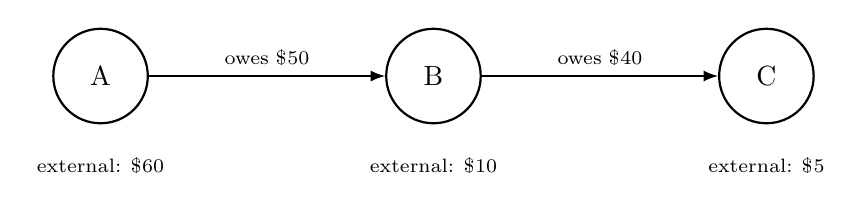
\begin{tikzpicture}[>=latex,thick,node distance=3.0cm]
        \node[draw,circle,minimum size=1.2cm] (a) {A};
        \node[draw,circle,minimum size=1.2cm,right=of a] (b) {B};
        \node[draw,circle,minimum size=1.2cm,right=of b] (c) {C};
        \draw[->] (a) -- node[above,font=\scriptsize] {owes \$50} (b);
        \draw[->] (b) -- node[above,font=\scriptsize] {owes \$40} (c);
        \node[below=0.3cm of a,font=\scriptsize] {external: \$60};
        \node[below=0.3cm of b,font=\scriptsize] {external: \$10};
        \node[below=0.3cm of c,font=\scriptsize] {external: \$5};
    \end{tikzpicture}
    \caption{A three-bank interbank obligation network. Bank A owes Bank B \$50; Bank B owes Bank C \$40; Bank C has no outstanding obligations. Each bank additionally holds the external (non-interbank) assets shown below it.}
    \label{fig:abm-contagion}
\end{figure}

In the baseline, no-shock case, every bank can pay its obligations in full: A's total resources are its $\$60$ of external assets (no one owes A anything), comfortably covering its $\$50$ obligation to B and leaving A with net worth $60-50=\$10$. B's resources are its $\$10$ of external assets plus the $\$50$ it receives from A, $\$60$ total, covering its $\$40$ obligation to C and leaving B with net worth $60-40=\$20$. C's resources are its $\$5$ of external assets plus the $\$40$ it receives from B, for a net worth of $\$45$. Total system-wide net worth is $10+20+45=\$75$.

Now suppose an external shock, a bad loan or a trading loss unrelated to the interbank network, destroys $\$45$ of Bank A's external assets, leaving A with only $\$15$. Recomputing the clearing vector: A's resources are now just $\$15$ against its $\$50$ obligation, so A pays only $\min(15,50)=\$15$ to B, a default with a $30\%$ recovery rate, leaving A with net worth $\$0$. B's resources are its own $\$10$ of external assets plus only $\$15$ from A (not the $\$50$ it was owed), $\$25$ total, against its own $\$40$ obligation to C; B can pay only $\min(25,40)=\$25$, so \emph{B also defaults}, with a $62.5\%$ recovery rate, even though B experienced no external shock of its own at all, its default is entirely a consequence of A's default. C's resources are its own $\$5$ plus only $\$25$ from B (not the $\$40$ it was owed), for a final net worth of $\$30$, down from $\$45$, a real loss even though C has no obligations to anyone and never itself defaults.

Table~\ref{tab:abm-contagion} summarizes the cascade. Total system-wide net worth falls from $\$75$ to $0+0+30=\$30$, a system-wide loss of exactly $\$45$, precisely equal to the size of the original shock: nothing about the network creates or destroys value, it only redistributes a single institution's loss across every institution downstream of it, in a pattern that would be invisible to a stress test of Bank A's portfolio in isolation.

\begin{table}[htbp]
\centering
\caption{The default cascade following a \$45 shock to Bank A's external assets (all figures in \$)}
\label{tab:abm-contagion}
\begin{tabular}{lrrrrrr}
\toprule
Bank & External (shocked) & Owed & Received & Paid & Net worth (baseline) & Net worth (shocked) \\
\midrule
A & 15 & 50 & 0  & 15 & 10 & 0 \\
B & 10 & 40 & 15 & 25 & 20 & 0 \\
C & 5  & 0  & 25 & 0  & 45 & 30 \\
\bottomrule
\end{tabular}
\end{table}

\section{Case Vignette: The Bank of England's RAMSI Model}
\index{Bank of England RAMSI model}

The contagion mechanism worked by hand in Section~\ref{sec:abm-contagion} is not merely a textbook simplification; it is a simplified version of machinery central banks actually use. Following the 2008 financial crisis, whose Gaussian-copula CDO mispricing Chapter 9 examines in detail, the Bank of England developed RAMSI (the Risk Assessment Model for Systemic Institutions), an agent-based model in which each major UK bank is represented as an agent with its own balance sheet, subject to macroeconomic shocks, interbank exposures, and behavioral responses such as fire-selling assets or curtailing lending under stress, precisely the kind of network-level cascade Section~\ref{sec:abm-contagion}'s three-bank example illustrates at a far larger and more realistic scale.

What makes RAMSI genuinely agent-based, rather than simply a larger version of Section~\ref{sec:abm-contagion}'s clearing-vector calculation, is that its banks do not only default mechanically when they cannot meet an obligation; they also take deliberate, self-protective actions in response to stress before default, exactly the kind of individually reasonable but collectively destabilizing behavior Section~\ref{sec:abm-why}'s Schelling and Flash Crash discussions both illustrate. A bank whose capital buffer is eroding might sell assets to raise cash, depressing the market price of those assets for every other bank holding the same asset class, a channel with no counterpart in the pure balance-sheet cascade of Section~\ref{sec:abm-contagion}, since nothing there let a bank's response feed back into the market prices other banks' own balance sheets depend on. This distinction matters practically: a pure Eisenberg-Noe network captures what regulators call first-round, direct contagion (a defaulted counterparty's unpaid obligations), while RAMSI-style behavioral responses capture second-round, indirect contagion (a healthy bank's own precautionary actions damaging other healthy banks), and post-crisis research consistently finds that second-round effects of this kind can be larger than the first-round direct losses they were triggered by, a finding no version of the three-bank chain or hub-and-spoke examples above, both purely first-round mechanisms, can reproduce on their own.

RAMSI and its successors are used to stress-test the UK banking system as a network rather than one institution at a time, directly extending the single-portfolio stress-testing framework of Chapter 8 to account for exactly the kind of contagious, second-round loss the worked example above shows a purely institution-by-institution stress test would miss entirely: in that example, a stress test of Bank B alone, which received no direct shock, would have reported B as perfectly healthy, right up until it wasn't. Other central banks and the IMF have developed comparable agent-based systemic-risk tools, and the approach is now a standard, if still specialized, part of the macroprudential regulator's toolkit alongside the more familiar single-institution VaR and stress-testing methods Chapter 8 covers.

\section[Agent-Based Models versus Multi-Agent Reinforcement Learning]{Agent-Based Models versus Multi-Agent Reinforcement Learning: Fixed Rules versus Learned Behavior}
\label{sec:abm-vs-marl}

Chapter 17's discussion of multi-agent dynamics observes that a reinforcement-learning agent trained against a static, historical simulator implicitly assumes every other participant's behavior stays fixed, an assumption the Flash Crash's hot-potato effect shows can fail badly in practice. Agent-based models and multi-agent reinforcement learning (MARL) are best understood as two different responses to that same observation, rather than as competitors. An ABM specifies each agent's behavioral rule directly, fundamentalist, chartist, zero-intelligence, and asks what emerges from many such fixed rules interacting; a MARL system instead lets each agent's behavior itself be learned, typically through the same Q-learning or policy-gradient machinery Chapter 17 develops, adapting to the other agents' evolving behavior rather than following a rule fixed in advance. The ABM approach trades away realism about how real traders learn and adapt in exchange for transparency and tractability, every agent's rule in this chapter's examples is a single, interpretable equation, while MARL trades that transparency away for the possibility of agents that behave more like real, adaptive market participants, at the cost of the training instability and weak convergence guarantees Chapter 17 already flags as MARL's central open problem. A growing body of research combines the two directly, building ABMs in which some or all agents follow reinforcement-learning policies rather than fixed behavioral rules, using the ABM's simulated market as exactly the kind of training environment Chapter 17's execution and market-making sections already rely on, an active research direction rather than a settled methodology. Table~\ref{tab:abm-vs-marl} summarizes the practical tradeoffs a modeler actually faces when choosing between the two.

\begin{table}[htbp]
\centering
\caption{Agent-based models (fixed rules) versus multi-agent reinforcement learning (learned behavior)}
\label{tab:abm-vs-marl}
\begin{tabular}{p{2.8cm}p{5.0cm}p{5.0cm}}
\toprule
 & Agent-based model & Multi-agent reinforcement learning \\
\midrule
Agent behavior     & Fixed, hand-specified rule            & Learned via Chapter 17's Q-learning or policy-gradient methods \\
Interpretability   & High: every rule is a single, readable equation & Low: behavior is implicit in a trained policy's weights \\
Adaptivity         & None, unless the modeler adds explicit switching (Section~\ref{sec:abm-fundamentalist-chartist}) & Agents adapt continuously to each other's evolving behavior \\
Convergence guarantees & Not applicable; the model is simulated, not trained & Weak once multiple agents learn simultaneously (Chapter 17) \\
Computational cost & Low to moderate                        & High, and grows sharply with agent count \\
Typical role in this book & Exploring what mechanisms are capable of producing an observed pattern (Section~\ref{sec:abm-calibration}) & Training a single production policy against a realistic simulated environment \\
\bottomrule
\end{tabular}
\end{table}

\subsection*{A Worked Example: A Learning Seller in the Double Auction}

To make the ABM-versus-MARL distinction concrete rather than only abstract, reconsider Section~\ref{sec:abm-zi}'s double auction, but replace one zero-intelligence seller with a seller who learns, in the same trial-and-error spirit as Chapter 17's bandit examples. Each round, a new buyer arrives with a valuation drawn from $\{45,50,55,60,65\}$ with equal probability, facing a seller with cost $\$40$ choosing between two fixed ask levels: Arm H (ask $\$58$) or Arm Lo (ask $\$47$). A trade occurs whenever the ask is at or below the buyer's valuation, earning the seller a profit of ask minus cost; a rejected ask earns nothing. The true expected profit of each arm, unknown to the seller but computable directly from the valuation distribution, is
\begin{equation*}
E[\text{profit}_H] = \Pr(v\ge 58)\times(58-40) = \tfrac{2}{5}\times18 = 7.2, \qquad E[\text{profit}_{Lo}] = \Pr(v\ge 47)\times(47-40) = \tfrac{4}{5}\times7 = 5.6,
\end{equation*}
so Arm H, despite trading less than half as often, is actually the better arm: its larger profit per trade more than compensates for its lower fill rate, a genuinely non-obvious tradeoff that neither arm's raw trade frequency reveals on its own.

The learning seller explores both arms twice (rounds 1 through 4, alternating H, Lo, H, Lo) and then plays greedily, choosing whichever arm has the higher running-average realized profit so far. Table~\ref{tab:abm-bandit} traces one representative 12-round history. After the four exploration rounds, Arm H's running average stands at $\$18.00$ against Arm Lo's $\$7.00$, so the seller plays Arm H for the remainder of the sequence, exactly matching the true optimal choice, and its running average, noisy at first, drifts down toward the true value of $\$7.2$ as more rounds accumulate.

\begin{table}[htbp]
\centering
\caption{One 12-round history of the learning seller in the double auction}
\label{tab:abm-bandit}
\begin{tabular}{rrlrrr}
\toprule
Round & Buyer value & Arm played & Profit & Avg.\ profit, H & Avg.\ profit, Lo \\
\midrule
1  & 60 & H  & 18 & 18.00 & --   \\
2  & 65 & Lo & 7  & 18.00 & 7.00 \\
3  & 60 & H  & 18 & 18.00 & 7.00 \\
4  & 60 & Lo & 7  & 18.00 & 7.00 \\
5  & 65 & H  & 18 & 18.00 & 7.00 \\
6  & 65 & H  & 18 & 18.00 & 7.00 \\
7  & 50 & H  & 0  & 14.40 & 7.00 \\
8  & 50 & H  & 0  & 12.00 & 7.00 \\
9  & 65 & H  & 18 & 12.86 & 7.00 \\
10 & 60 & H  & 18 & 13.50 & 7.00 \\
11 & 65 & H  & 18 & 14.00 & 7.00 \\
12 & 50 & H  & 0  & 12.60 & 7.00 \\
\bottomrule
\end{tabular}
\end{table}

This is the ABM-versus-MARL distinction from Table~\ref{tab:abm-vs-marl} made concrete within a single example: every other seller in Section~\ref{sec:abm-zi} follows a fixed rule (draw a random ask, full stop), while this one adapts its behavior based on realized experience, exactly the shift from a specified rule to a learned policy that separates the two columns of that table. It is also worth being honest about what a single 12-round history does and does not show: this particular valuation sequence happened to make both exploration draws for Arm H land on high-valuation buyers, letting the seller lock onto the correct arm immediately; a less fortunate exploration phase could just as easily have left the seller with a misleadingly low early estimate for the better arm, favoring the worse one for a while, exactly the explore-exploit tension that makes reinforcement learning harder in practice than this one clean run suggests.

\subsection*{A Worked Example: Discrete-Choice Switching Replaces the Fixed Threshold}
\label{sec:abm-discrete-choice}

The learning seller above replaces one agent's fixed rule with something learned; it is worth asking the same question of Section~\ref{sec:abm-stylized-facts}'s regime-switching market, where the population mix $(n_f,n_c)$ was allowed to evolve, but only according to a threshold rule handed down by the modeler, switch to the volatile regime whenever the last price move exceeds a fixed cutoff, not according to anything any fundamentalist or chartist actually experienced. Brock and Hommes's own mechanism, named in passing in Section~\ref{sec:abm-why} and Section~\ref{sec:abm-stylized-facts} and derived in full generality in this book's companion technical note on the Brock-Hommes model, replaces that external threshold with exactly the comparison a real trader would make: at every period, each strategy's population share updates according to a discrete-choice (logit) rule driven by that strategy's own recently realized profit, so the switching Section~\ref{sec:abm-stylized-facts} imposed from outside instead emerges from many individual agents each comparing two numbers and choosing, probabilistically, whichever strategy has recently paid off better.

Reusing Section~\ref{sec:abm-fundamentalist-chartist}'s market exactly, $p_f=100$, $\alpha=0.3$, $\beta=1.0$, $\lambda=1.5$, $p_{-1}=93$, $p_0=95$, define each strategy's realized profit at $t$ as the price change just observed times the demand that strategy would have submitted one period earlier,
\begin{equation*}
\pi_{f,t} = (p_t-p_{t-1})\,d^f_{t-1}, \qquad \pi_{c,t} = (p_t-p_{t-1})\,d^c_{t-1},
\end{equation*}
and update the fundamentalist population share by the binary logit rule
\begin{equation*}
n_{f,t} = \frac{e^{\theta \pi_{f,t}}}{e^{\theta\pi_{f,t}}+e^{\theta\pi_{c,t}}}, \qquad n_{c,t}=1-n_{f,t},
\end{equation*}
where $\theta\ge0$ is the intensity of choice (written $\theta$ here rather than the technical note's own $\beta$, to avoid clashing with this chapter's already-established chartist coefficient $\beta$): $\theta=0$ freezes the population at whatever split it started with regardless of performance, while a large $\theta$ sends nearly the entire population to whichever strategy did even slightly better last period.

Starting from an uninformed $n_{f,0}=n_{c,0}=0.5$, no fitness history yet exists to compare, and $\theta=0.5$, Table~\ref{tab:abm-discrete-choice} works the first three periods by hand.

\begin{table}[htbp]
\centering
\caption{Discrete-choice switching ($\theta=0.5$) replacing Section~\ref{sec:abm-stylized-facts}'s fixed threshold. Each period's population shares are computed from the fitness realized over the immediately preceding period, then used to set that period's aggregate demand.}
\label{tab:abm-discrete-choice}
\begin{tabular}{lrrrrrrr}
\toprule
$t$ & $p_t$ & $n_{f,t}$ & $n_{c,t}$ & $d^f_t$ & $d^c_t$ & $D_t$ & $p_{t+1}$ \\
\midrule
0 & 95.000  & 0.500 & 0.500 & 1.500    & 2.000 & 1.750 & 97.625 \\
1 & 97.625  & 0.342 & 0.658 & 0.713    & 2.625 & 1.972 & 100.583 \\
2 & 100.583 & 0.056 & 0.944 & $-0.175$ & 2.958 & 2.783 & 104.757 \\
\bottomrule
\end{tabular}
\end{table}

The first period's fitness gap is already informative: with $\Delta p_1=2.625$, the chartist demand submitted the period before, $d^c_0=2.0$, earned a realized profit of $\pi_{c,1}=2.625\times2.0=5.250$, against the fundamentalist's $\pi_{f,1}=2.625\times1.5=3.938$; chartists were not merely more numerous, they were genuinely more profitable, since their demand happened to be better aligned with the up-move that materialized. The logit rule converts this into $n_{c,1}=0.658$, already sitting at the very edge of the exact critical threshold $n_c^{*}\approx0.667$ Section~\ref{sec:abm-fundamentalist-chartist} derived analytically for this same $\lambda$ and $\beta$. One further period of chartist outperformance, $\pi_{c,2}=7.764$ against $\pi_{f,2}=2.107$, pushes the population decisively past that threshold to $n_{c,2}=0.944$, and the price increments confirm the market has genuinely crossed into the unstable regime: $\Delta p_1=2.625$, $\Delta p_2=2.958$, $\Delta p_3=4.174$, growing rather than shrinking, exactly Scenario B's explosive signature, but reached here with no threshold rule written into the model at all, only individual agents comparing two realized numbers each period and updating a choice probability accordingly.

This result is worth placing carefully within Table~\ref{tab:abm-vs-marl}'s ABM-versus-MARL contrast rather than folded unchanged into either column. It is not Chapter 17's Q-learning: no agent here maintains a state-action value table or bootstraps a return estimate the way the learning seller above does. It is closer to a population-level analogue of the same idea, an evolutionary or replicator dynamic in which strategies that recently paid off are simply used by more of the population next period. That distinction matters for interpretability: a single logit population share is still a single number a reader can audit by hand, exactly as this worked example just did, in a way a trained neural-network policy's weights are not, so discrete-choice switching sits closer to the transparent, fixed-rule end of Table~\ref{tab:abm-vs-marl}'s spectrum than the learning seller does, even though both replace a rule the modeler would otherwise have to impose with something the agents themselves determine. The companion technical note develops this same mechanism with a fully specified CARA-utility demand system rather than this chapter's simpler linear demand rules, and derives, in closed form, the equilibrium population share and its exact stability condition as a function of the intensity of choice, a genuine analogue of this section's $n_c^{*}$, but expressed as a threshold on $\theta$ rather than directly on the population share, since in that richer model the population share is itself an endogenous function of $\theta$ rather than a free parameter the modeler sets. Brock and Hommes's own result goes one step further still: beyond that critical intensity of choice, the market does not merely become unstable in the sense this section's numbers illustrate, its dynamics undergo a period-doubling bifurcation into deterministic chaos, price behavior that looks statistically indistinguishable from noise despite being generated by a fully deterministic, rational system, the technical note's own ``rational route to randomness.'' A reader who wants that fully rigorous derivation, rather than this section's numerical illustration of the same underlying idea, should turn to the technical note directly.

\section{Calibrating and Validating Agent-Based Models}
\label{sec:abm-calibration}

Chapter 6 validates a model by holding out data the model never saw during training and checking its predictions against it, a well-defined procedure precisely because the model produces a specific, checkable prediction for each held-out observation. Agent-based models are far harder to validate in this sense, because an ABM does not produce a single prediction to check against a single observation; it produces an entire simulated history, and the object of interest is usually a qualitative or statistical property of that history, does it produce fat tails, does it produce a plausible contagion cascade, not a point forecast. The standard approach, the method of simulated moments\index{Method of Simulated Moments}, instead chooses the model's free parameters (here, quantities like $\alpha$, $\beta$, $\lambda$, and the population-switching rule governing $n_f$ and $n_c$) to make the simulated data's statistical moments, its volatility, its kurtosis, its autocorrelation structure, match the same moments computed from real market data as closely as possible, rather than maximizing a likelihood the way Chapter 6's models typically do.

This procedure carries a genuine risk that deserves the same skepticism Chapter 6 applies to overfitting: an ABM with enough free behavioral parameters can often be tuned to match almost any target set of stylized facts, which demonstrates that the model is flexible, not that its particular mechanism, fundamentalists and chartists switching by relative profitability, say, is the true explanation for why real markets exhibit those facts. A model that reproduces fat tails is not thereby confirmed; a different ABM, or even a different set of parameters within the same ABM, might reproduce the same fat tails through an entirely different mechanism. This is a substantive limitation, not a minor technicality, and is the central reason agent-based models are generally used in this book's spirit, as a tool for exploring what mechanisms are capable of producing an observed pattern, alongside real institutional case studies like the Flash Crash and the RAMSI vignette above, rather than as a forecasting tool to be validated the way Chapter 6's classifiers and Chapter 7's time-series models are.

\subsection*{Concretely: Matching a Target Moment}

Section~\ref{sec:abm-stylized-facts}'s regime-switching simulation happened to produce a Pearson kurtosis of $5.23$ from a switching threshold of $0.25$; nothing forced that particular value. Method-of-simulated-moments calibration treats the switching threshold (and any of the model's other free parameters) as a dial to search over, re-running the simulation at several threshold values and recording the resulting kurtosis, exactly as Table~\ref{tab:abm-msm-sweep} does.

\begin{table}[htbp]
\centering
\caption{Simulated kurtosis as a function of the switching threshold (500 periods, otherwise identical to Section~\ref{sec:abm-stylized-facts})}
\label{tab:abm-msm-sweep}
\begin{tabular}{rr}
\toprule
Switching threshold & Pearson kurtosis \\
\midrule
0.15 & 3.82 \\
0.20 & 3.91 \\
0.25 & 5.23 \\
0.30 & 6.62 \\
0.35 & 11.64 \\
\bottomrule
\end{tabular}
\end{table}

The direction is worth pausing on, because it is not the one intuition suggests first: kurtosis \emph{rises} as the threshold rises, that is, as the volatile regime becomes \emph{harder} to trigger, not easier. A low threshold puts the market into the volatile regime often, which raises overall variance but makes the two regimes blend into one another rather than standing sharply apart; a high threshold makes the volatile regime rare, so on the infrequent occasions it does trigger, it produces a small number of sharp outliers against an otherwise calm baseline, exactly the mixture-of-a-common-calm-regime-and-a-rare-extreme-regime structure that drives kurtosis up. Suppose an analyst wanted the simulation to match a specific real asset's historically observed kurtosis of $6.0$: Table~\ref{tab:abm-msm-sweep} shows the threshold value that comes closest is $0.30$, landing at $6.62$, a small overshoot that a finer search between $0.25$ and $0.30$ would narrow further. Crucially, finding a threshold that approximately matches $6.0$ would establish only that this particular mechanism, among what is likely a wide range of other threshold values, population-share assumptions, or entirely different ABM structures, is \emph{capable} of producing that kurtosis, not that real traders actually switch strategies according to anything resembling this rule, and, as this reversed direction illustrates concretely, not that the calibrated parameter's economic interpretation, ``how readily the market panics,'' behaves the way casual intuition about it would suggest. That gap, between matching a moment and confirming a mechanism, is precisely Section~\ref{sec:abm-calibration}'s central caution, restated here in terms of real, computed numbers rather than in the abstract.

\section{Advanced Topics: Network Topology and the Limits of a Simple Chain}
\label{sec:abm-advanced}

Section~\ref{sec:abm-contagion}'s three-bank example deliberately used the simplest possible network, a single chain, in which every bank has exactly one creditor and at most one debtor. Real interbank networks look nothing like a chain: they are typically core-periphery structures, a small number of large, heavily interconnected banks at the core, surrounded by many smaller banks each connected mainly to the core rather than to each other, and the shape of that network turns out to matter for how a shock propagates, not merely how large the shock is. Acemoglu, Ozdaglar, and Tahbaz-Salehi's widely cited ``robust-yet-fragile'' result formalizes an initially counterintuitive finding: for small shocks, a more densely connected network is more stable, since each bank's exposure to any single counterparty's distress is diluted across many other relationships, exactly the diversification logic behind Chapter 10's portfolio theory. But past a certain shock size, that same dense interconnection reverses roles entirely, turning into a contagion channel that transmits a large shock further and faster than a sparser network would have, because a large loss concentrated at one interconnected core bank now has many more downstream counterparties to infect than it would in a sparse network.

\subsection*{A Worked Example: Chain versus Hub-and-Spoke}

Consider replacing Section~\ref{sec:abm-contagion}'s chain with a hub-and-spoke network hit by exactly the same $\$45$ shock, so the two topologies can be compared directly. A hub bank $H$ owes $\$30$ to each of three peripheral banks $P_1$, $P_2$, $P_3$ ($\$90$ owed in total), $H$ holds $\$100$ of external assets, and each $P_i$ holds $\$5$ of external assets and has no obligations of its own. In the baseline, $H$ pays all three peripherals in full, leaving $H$ with net worth $100-90=\$10$ and each $P_i$ with net worth $5+30=\$35$, for a total system net worth of $10+3(35)=\$115$.

Now apply the same $\$45$ shock used against Bank A in Section~\ref{sec:abm-contagion}, this time to $H$'s external assets, reducing $H$'s resources to $\$55$ against its $\$90$ total obligation. Eisenberg-Noe clearing requires $H$ to pay each equally senior creditor the same pro-rata share of what it has: $H$ can cover only $55/90=61.1\%$ of what it owes, so each $P_i$ receives $\$18.33$ instead of the full $\$30$. $H$'s net worth falls to $55-55=\$0$, a default, exactly as Bank A's did in the chain, but now every peripheral bank absorbs a slice of the loss simultaneously rather than sequentially: each $P_i$ ends with net worth $5+18.33=\$23.33$, down from $\$35$, a $33.3\%$ loss for every single one of the three peripherals, incurred in the same instant. Table~\ref{tab:abm-hub-spoke} summarizes both networks side by side. Total system-wide loss is exactly $\$45$ in both cases, matching the shock size regardless of topology, a general property of this clearing mechanism with no bankruptcy costs, so topology does not change how much value a shock destroys in total; what it changes entirely is how that loss is distributed. The chain concentrates outright default onto two institutions in sequence (A, then B), with C absorbing a comparatively modest, once-removed spillover; the hub-and-spoke network concentrates outright default onto a single institution, the hub itself, while spreading a real but survivable loss simultaneously across every peripheral bank, none of which technically defaults, since none had any obligation to fail to meet, but all three are meaningfully weaker. Neither topology is simply ``worse''; which one a regulator should worry about more depends on whether the greater concern is a small number of outright failures cascading through a chain of counterparties, or a single well-connected institution's distress passing a real loss simultaneously to everyone depending on it, exactly the kind of topology-dependent judgment RAMSI-style network models are built to inform.

\begin{table}[htbp]
\centering
\caption{The same \$45 shock, chain versus hub-and-spoke}
\label{tab:abm-hub-spoke}
\begin{tabular}{lrrr}
\toprule
Network & Institutions defaulting outright & Total system loss & Loss distribution \\
\midrule
Chain (Section~\ref{sec:abm-contagion}) & 2 of 3 (A, then B) & \$45 & Concentrated, sequential \\
Hub-and-spoke (above) & 1 of 4 (H only) & \$45 & Diffuse, simultaneous \\
\bottomrule
\end{tabular}
\end{table}

A full treatment of how network topology governs the robust-yet-fragile transition would require simulating the clearing-vector calculation across many more network structures and shock sizes than the two compared here, exactly the kind of large-scale agent-based exercise real central-bank models like RAMSI are built to run.

\section{A Practical Workflow for Building an Agent-Based Model}
\label{sec:abm-workflow}

Every example in this chapter, despite covering three quite different applications, market efficiency, price dynamics, and financial contagion, followed the same underlying workflow, worth stating explicitly as a template for building a new ABM from scratch, and, more fundamentally, as a concrete answer to what it actually means, step by step, to ask Table~\ref{tab:abm-paradigms}'s question, ``what pattern emerges from many interacting rules,'' rather than fitting a function to data or training a policy against an environment.

\begin{enumerate}
    \item \textbf{Specify the agents and their behavioral rules.} Decide what types of agents populate the model (zero-intelligence traders, fundamentalists and chartists, banks in a network) and write down each type's rule as an explicit function of the current market state, exactly as Sections~\ref{sec:abm-zi} through~\ref{sec:abm-contagion} did with a single equation or a short block of code per agent type.
    \item \textbf{Specify the market mechanism.} Decide how individual agent actions aggregate into a new market state: a double-auction clearing rule, a price-impact equation, an Eisenberg-Noe clearing vector. This is the second box in Figure~\ref{fig:abm-loop}'s simulation loop, and is usually the piece of the model most directly grounded in institutional fact rather than behavioral assumption.
    \item \textbf{Choose free parameters and initial conditions.} Every worked example above had a handful of free parameters, $\alpha$, $\beta$, $\lambda$, the population shares $(n_f,n_c)$, a switching threshold, that are not derived from anything but simply set by the modeler. Report these explicitly and be prepared to defend each one, since Section~\ref{sec:abm-calibration}'s calibration critique applies to every one of them.
    \item \textbf{Simulate forward and collect statistics.} Run the loop for enough periods that the statistic of interest, an efficiency percentage, a variance ratio, a kurtosis, a default count, stabilizes, and report it alongside the raw simulated series wherever possible, exactly as this chapter's companion notebook does for all four worked examples.
    \item \textbf{Calibrate against real data if a real comparison is available.} Where a target real-world moment exists, Section~\ref{sec:abm-calibration}'s method of simulated moments searches over the free parameters from step 3 until simulated and real moments match as closely as possible.
    \item \textbf{Interpret the result as a candidate mechanism, not a confirmed explanation.} A model that reproduces a target pattern has shown that its mechanism is \emph{capable} of producing that pattern; Section~\ref{sec:abm-calibration}'s central caution, restated once more here because it is the single most important methodological point in this chapter, is that this is weaker evidence than a validated prediction from Chapter 6's train-test framework, and should be presented and used accordingly.
\end{enumerate}

\section{Challenges in Agent-Based Modeling for Finance}

Agent-based models face several challenges that are worth naming explicitly, since they explain why ABMs remain a specialized tool rather than a default modeling choice throughout this book. Computational cost is real: simulating a large, heterogeneous population over many time steps, especially when agents themselves are learned via the reinforcement-learning methods of Section~\ref{sec:abm-vs-marl}, can be far more expensive than fitting a single closed-form or statistical model to historical data. Every worked example in this chapter used only two to four agents specifically because a hand-checkable illustration has to; a research-grade financial ABM more typically simulates thousands to millions of agents, and, since every agent must be updated every period, cost grows at best linearly and often worse than linearly in both agent count and simulated horizon, a scaling concern this book's other methods, a single fitted regression or a single trained network regardless of dataset size, mostly do not share. General-purpose ABM frameworks such as Mesa (Python) and NetLogo exist specifically to manage this complexity, but building and validating a large-scale financial ABM remains a substantially larger engineering undertaking than fitting one of Chapter 6's models to a comparable dataset. Calibration and validation, discussed in Section~\ref{sec:abm-calibration}, remain genuinely unresolved problems: the method of simulated moments can match target statistics without establishing that the underlying mechanism is correct, and there is no equivalent of Chapter 6's clean train-test split for an entire emergent history. Reproducibility across studies is weaker than in most of this book's other methods, since two research groups' ABMs of, nominally, the same phenomenon frequently differ in dozens of implementation details, agent count, order of updates, tie-breaking rules, that are rarely fully specified and can materially change the results. Finally, regulatory and industry acceptance lags behind the academic literature: RAMSI-style tools have earned a place in the macroprudential toolkit specifically because central banks can defend their assumptions in a way appropriate to their narrow, systemic-risk purpose, but agent-based models remain far from a routine part of the model validation and governance framework Chapter 13's three-lines-of-defense discipline and Chapter 16's explainability toolkit were built around, largely because a rule-based simulation of thousands of interacting agents is a fundamentally harder object to explain to a validator, or to a regulator, than a single fitted regression or classifier.

None of these challenges is a reason to avoid agent-based models; they are reasons to be precise about what a given ABM has and has not shown, exactly the discipline Section~\ref{sec:abm-workflow}'s final step asks for. A model that reproduces the Flash Crash's hot-potato dynamics, or the fat tails of Section~\ref{sec:abm-stylized-facts}'s regime-switching simulation, or RAMSI's contagion cascades, is a genuine, useful demonstration that a specific, named mechanism is \emph{sufficient} to produce an observed pattern, valuable evidence in its own right, and often the only tractable way to reason about emergent phenomena at all. It is simply not, on its own, evidence that the mechanism is \emph{necessary}, the one true explanation among the many candidate mechanisms that might produce the same pattern, and every application in this chapter should be read with that distinction in mind.

\section{Key Takeaways}

\begin{itemize}
    \item Agent-based models simulate a population of heterogeneous, boundedly rational agents interacting repeatedly, and treat the aggregate pattern that emerges, efficiency, a bubble, a cascade, as the object of study, in contrast to this book's representative-agent equilibrium models and data-fitted statistical models.
    \item Market efficiency can emerge from a trading mechanism itself rather than from participant sophistication: zero-intelligence traders bidding at random within budget constraints, cleared through an ordinary double auction, recovered the fully efficient trade in this chapter's worked example.
    \item The same market mechanism can produce either smooth convergence to fundamental value or a self-reinforcing, explosive bubble, depending only on the population mix of fundamentalist and chartist traders, holding every other parameter fixed.
    \item Heterogeneous-agent models can reproduce fat tails and volatility clustering as an emergent consequence of strategy switching, rather than by directly imposing an autoregressive variance structure the way Chapter 7's GARCH models do: this chapter's 500-period simulation produced a $7.14\times$ variance ratio between regimes, a Pearson kurtosis of $5.23$ against a Gaussian benchmark of $3.0$, and a squared-return autocorrelation of $0.761$ at lag one, from nothing more than two fixed behavioral rules switching in and out of dominance.
    \item A clearing-vector approach to interbank obligations, the same logic underlying the Bank of England's RAMSI model, can show one institution's shock cascading into a second institution's default even when that second institution received no direct shock at all, a genuinely systemic risk a single-institution stress test cannot see.
    \item Agent-based models are far harder to calibrate and validate than this book's other methods, since matching a target set of statistical moments demonstrates flexibility, not that the model's particular mechanism is the true explanation for the observed pattern.
    \item Network topology shapes contagion independently of shock size: the ``robust-yet-fragile'' result shows dense interconnection dampens small shocks through diversification but can transmit large shocks further and faster than a sparser network would; the same \$45 shock produced two outright defaults in a chain network but only one, spread more diffusely, in a hub-and-spoke network of the same total size.
    \item The fundamentalist-chartist market's stability is governed by a single exact threshold, $n_c^{*}=1/(\lambda\beta)$: below it the price converges, above it a bubble grows without bound, and near it convergence becomes oscillatory rather than smooth, a sharp regime change from one parameter crossing a critical value.
    \item Agent-based models answer a third kind of question this book's other two paradigms do not: not ``what function best fits this data'' (Chapter 6) or ``what action sequence maximizes reward in this environment'' (Chapter 17), but ``what pattern emerges when many simple, interacting rules are simulated together.''
    \item Even a calibrated parameter's economic interpretation can run against intuition: raising the fundamentalist-chartist model's switching threshold, making the volatile regime \emph{harder} to trigger rather than easier, raised simulated kurtosis from $3.82$ to $11.64$ across a real parameter sweep, the opposite of the direction naive intuition suggests, underscoring why a calibrated ABM's internal mechanism should never be trusted just because its output moments look right.
    \item A fixed-rule ABM and a learning agent can occupy the exact same market: replacing one zero-intelligence seller with a simple trial-and-error learner that tracks realized profit converged on the true better strategy in this chapter's worked example, but a single unlucky exploration phase can just as easily lock a purely greedy learner onto the wrong one permanently, with no further exploration to self-correct it.
    \item A market's switching threshold can be crossed by assumption or by learning: Section~\ref{sec:abm-stylized-facts}'s regime switch was a rule the modeler imposed from outside, while Section~\ref{sec:abm-discrete-choice}'s discrete-choice mechanism let the population cross the identical $n_c^{*}\approx0.667$ threshold on its own, purely because agents kept reallocating toward whichever strategy had just earned more, reaching $n_{c,2}=0.944$ and an accelerating price after only two periods of chartist outperformance.
\end{itemize}

\section{Suggested Exercises}

\begin{enumerate}
    \item Using the zero-intelligence double-auction setup of Section~\ref{sec:abm-zi}, suppose buyer 2's random bid is $b_2=\$49$ instead of $\$30$, with every other draw unchanged. Recompute the clearing outcome and explain, in terms of total realized surplus, whether the market mechanism still selects the efficient allocation.
    \item Section~\ref{sec:abm-fundamentalist-chartist} derives the stability threshold $n_c^{*}=1/(\lambda\beta)$ for $\lambda=1.5$, $\beta=1.0$. Recompute $n_c^{*}$ for $\beta=2.0$ instead, holding $\lambda=1.5$ fixed, and use the companion notebook to confirm your answer by simulating the market just above and just below the new threshold.
    \item Extend the three-bank contagion network of Section~\ref{sec:abm-contagion} by adding a fourth bank, D, to whom Bank C owes \$20, with D holding \$15 of external assets and no other obligations. Recompute the clearing vector under the same \$45 shock to Bank A's external assets, and report whether the cascade reaches D.
    \item Section~\ref{sec:abm-advanced}'s hub-and-spoke example used three peripheral banks. Redo the calculation with six peripheral banks instead, keeping the hub's total obligation at \$90 (so each peripheral is now owed \$15) and its external assets at \$100, under the same \$45 shock. Report each peripheral's percentage loss and compare it to the three-peripheral case's $33.3\%$, and explain the direction of the difference.
    \item Section~\ref{sec:abm-calibration} argues that matching a target set of statistical moments does not confirm an ABM's underlying mechanism. Propose one additional form of evidence, beyond matching moments, that would make you more confident a particular agent-based mechanism is the right explanation for an observed market phenomenon.
    \item Using the companion notebook's regime-switching simulation, lower the switching threshold from $0.25$ to $0.15$ and re-run the $500$-period simulation. Report the new variance ratio and kurtosis, and explain, in terms of how often the market now enters the volatile regime, why the direction of the change makes sense.
    \item Section~\ref{sec:abm-vs-marl}'s learning seller happened to explore into a lucky sequence. Recompute its running averages after exploration if rounds 1 through 4 instead see buyer values $50, 50, 50, 50$ (using the companion notebook to check your work), report which arm the seller would then play for the rest of the sequence, and explain why this outcome is a genuine failure of the explore-exploit process rather than merely bad luck that later self-corrects.
    \item Using Section~\ref{sec:abm-discrete-choice}'s discrete-choice market, recompute $n_{f,1}$, $n_{c,1}$, $n_{f,2}$, and $n_{c,2}$ with a lower intensity of choice, $\theta=0.2$ instead of $0.5$, holding every other parameter and the same $p_{-1}=93$, $p_0=95$ fixed, and report the first period at which $n_{c,t}$ exceeds the critical threshold $n_c^{*}\approx0.667$ derived in Section~\ref{sec:abm-fundamentalist-chartist}, comparing it to the $\theta=0.5$ case worked in the text, where the threshold was already exceeded after a single period.
    \item \textbf{Challenge (real data).} Download the BIS locational banking statistics (the cross-border claims table, freely available at stats.bis.org with no registration required) for five or six reporting countries. (a) Treating each country's aggregate cross-border claims on the others as a simplified interbank exposure network, construct a liabilities matrix analogous to Section~\ref{sec:abm-contagion}'s three-bank example (using each country's claims on another as that other country's liability), and compute the Eisenberg-Noe clearing vector following an assumed shock that wipes out 10\% of one country's external, non-interbank assets. (b) Compare the resulting loss cascade to this chapter's toy three-bank result, and discuss whether the real network's exposures look more chain-like or more hub-and-spoke, referencing Section~\ref{sec:abm-advanced}'s topology comparison. (c) Explain one specific way in which country-aggregated BIS data understates the fragility of the true institution-level network (for example, netting across many banks within a country, or omitting domestic interbank exposures entirely), and describe, referencing this chapter's RAMSI case vignette, what institution-level supervisory exposure data a central bank could use to close that gap.
\end{enumerate}

\section{Further Reading}

\begin{itemize}
    \item Schelling, T. C., ``Dynamic Models of Segregation,'' \emph{Journal of Mathematical Sociology}. The original checkerboard segregation model discussed in Section~\ref{sec:abm-why}, the earliest and best-known agent-based model outside finance.
    \item Arthur, W. B., Holland, J. H., LeBaron, B., Palmer, R., and Tayler, P., ``Asset Pricing Under Endogenous Expectations in an Artificial Stock Market,'' in \emph{The Economy as an Evolving Complex System II}. The Santa Fe Institute Artificial Stock Market discussed in Section~\ref{sec:abm-why}, widely regarded as the founding model of agent-based computational finance.
    \item Gode, D. K., and Sunder, S., ``Allocative Efficiency of Markets with Zero-Intelligence Traders,'' \emph{Journal of Political Economy}. The original zero-intelligence double-auction result worked through by hand in Section~\ref{sec:abm-zi}.
    \item Brock, W. A., and Hommes, C. H., ``A Rational Route to Randomness,'' \emph{Econometrica}. The performance-based strategy-switching framework underlying Section~\ref{sec:abm-fundamentalist-chartist}'s fundamentalist-chartist model.
    \item Lux, T., and Marchesi, M., ``Scaling and Criticality in a Stochastic Multi-Agent Model of a Financial Market,'' \emph{Nature}. An influential heterogeneous-agent model reproducing fat tails and volatility clustering, discussed in Section~\ref{sec:abm-stylized-facts}.
    \item Eisenberg, L., and Noe, T. H., ``Systemic Risk in Financial Systems,'' \emph{Management Science}. The clearing-vector framework for financial contagion worked through by hand in Section~\ref{sec:abm-contagion}.
    \item Acemoglu, D., Ozdaglar, A., and Tahbaz-Salehi, A., ``Systemic Risk and Stability in Financial Networks,'' \emph{American Economic Review}. The ``robust-yet-fragile'' network-topology result discussed in Section~\ref{sec:abm-advanced}.
    \item Zhang, K., Yang, Z., and Ba\c{s}ar, T., ``Multi-Agent Reinforcement Learning: A Selective Overview of Theories and Algorithms,'' in \emph{Handbook of Reinforcement Learning and Control}. A survey of the multi-agent reinforcement learning methods contrasted with fixed-rule agent-based models in Section~\ref{sec:abm-vs-marl}, including the convergence difficulties that arise once multiple agents learn simultaneously.
    \item Bank of England, ``RAMSI: A Top-Down Stress-Testing Model,'' Bank of England Working Paper. The real-world central-bank systemic-risk model discussed in the case vignette above.
    \item Axtell, R. L., and Farmer, J. D., ``Agent-Based Modeling in Economics and Finance: Past, Present, and Future,'' \emph{Journal of Economic Literature} 63(1): 197--287. A comprehensive, up-to-date survey of the field from two of its leading figures, and the best single starting point for a reader who wants to go beyond this chapter's introductory treatment.
    \item LeBaron, B., ``Agent-Based Computational Finance,'' in \emph{Handbook of Computational Economics}. An earlier survey of the agent-based finance literature specifically, including the calibration and validation challenges raised in Section~\ref{sec:abm-calibration}.
    \item Farmer, J. D., and Foley, D., ``The Economy Needs Agent-Based Modelling,'' \emph{Nature}. An argument, from two leading practitioners, for agent-based approaches as a complement to equilibrium modeling in macroeconomics and finance.
\end{itemize}

\end{document}
